\documentclass[a4paper,12pt]{article}
\usepackage[utf8]{inputenc}
\usepackage{geometry}
\usepackage{graphicx}
\usepackage{hyperref}
\hypersetup{
    colorlinks=true,
    linkcolor=blue,
    citecolor=blue,
    urlcolor=blue
}
\usepackage[style=ieee,backend=biber]{biblatex}
\usepackage{tikz} % Pentru logo
\usepackage{pgfplots} % Pentru grafice
\pgfplotsset{compat=1.18}
\geometry{margin=1in}

\addbibresource{docs/references.bib}

\title{Russia’s War on Ukraine: Human Rights and EU-NATO Silence \\ \large Blood in the Balance}
\author{Teodor Berger}
\date{May 2025}

\begin{document}

\maketitle

\begin{center}
    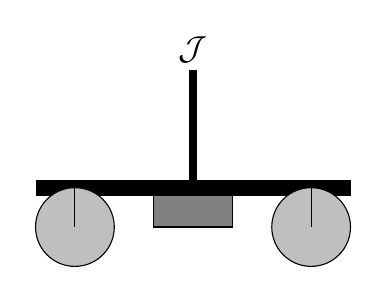
\begin{tikzpicture}[scale=0.5]
    % Baza cântarului
    \draw[fill=gray] (0,-1) rectangle (2,0);
    % Brațul cântarului
    \draw[line width=2mm] (-3,0) -- (5,0);
    % Suportul central
    \draw[line width=1mm] (1,0) -- (1,3);
    % Talere
    \draw[fill=lightgray] (-2,-1) circle (1);
    \draw[fill=lightgray] (4,-1) circle (1);
    % Lanțuri
    \draw (-2,0) -- (-2,-1);
    \draw (4,0) -- (4,-1);
    % Simbol justiție
    \node at (1,3.5) {\large $\mathcal{J}$};
\end{tikzpicture}
 % Include logo TikZ
\end{center}

\begin{abstract}
This report rigorously documents human rights violations committed by the Russian Federation in the Russo-Ukrainian War, alongside the strategic silence of international actors (EU, NATO, and others). Through verified data and moral analysis, it exposes the human cost of inaction and proposes actionable solutions for global responsibility.
\end{abstract}

\vspace{1em}
\noindent\textit{This report is available in English. For translations, consider using tools like DeepL or Google Translate.}

\section{Moral and Philosophical Introduction}
The sanctity of human life is non-negotiable. Yet, in the face of deliberate atrocities—targeted civilian attacks, forced deportations, and systematic torture—the international community’s silence becomes a form of complicity. This report begins with a moral question: How can the world justify inaction when lives are measured against geopolitical calculations? Drawing on ethical frameworks, from Kant’s categorical imperative to modern human rights principles, we argue that passivity in the face of aggression is not neutrality but a choice with devastating consequences \cite{un_2023}.

\section{Geopolitical Context}
The Russo-Ukrainian War cannot be understood without examining the historical and legal frameworks violated by the Russian Federation. Ukraine’s sovereignty, established after the dissolution of the Soviet Union in 1991, was repeatedly undermined by Russian actions, culminating in the 2014 annexation of Crimea and the full-scale invasion of 2022.

The Russian Federation’s actions contravene multiple international agreements:
\begin{itemize}
    \item \textbf{Charter of the United Nations (1945)}: Article 2(4) prohibits the use of force against the territorial integrity or political independence of any state \cite{un_charter}. Russia’s annexation of Crimea and military aggression in Ukraine directly violate this principle.
    \item \textbf{Helsinki Final Act (1975)}: Signed by the Soviet Union, this agreement commits signatories to respect the inviolability of frontiers and territorial integrity \cite{helsinki_1975}. Russia’s actions in Crimea and eastern Ukraine breach these commitments.
    \item \textbf{Memorandum on Security Assurances (Budapest, 1994)}: In exchange for Ukraine’s denuclearization, Russia, the United States, and the United Kingdom pledged to respect Ukraine’s sovereignty and territorial integrity \cite{budapest_1994}. Russia’s invasion constitutes a clear violation of this agreement.
\end{itemize}

\subsection{Breaching the 1991 Alma-Ata Protocol}
The Alma-Ata Declaration (1991), signed by Russia and 11 former Soviet republics, confirmed the dissolution of the USSR and mutual recognition of existing borders \cite{alma_ata_1991}. Russia’s invasion of Ukraine in 2014 and 2022 violates this foundational post-Soviet agreement, calling into question Moscow’s legal respect for its own commitments.

\subsection{Breaching the Geneva Conventions}
The Geneva Conventions of 1949 and their Additional Protocols mandate the protection of civilians, prisoners of war, and wounded during armed conflicts \cite{geneva_1949}. Russia’s deliberate attacks on civilian infrastructure (e.g., hospitals in Mariupol), torture of prisoners in occupied territories, and use of prohibited weapons like cluster munitions violate these obligations. These breaches, documented by the UN and Human Rights Watch, constitute war crimes and erode the foundational principles of international humanitarian law \cite{un_inquiry_2023, hrw_2023}.

The annexation of Crimea in 2014, followed by Russia’s support for separatist movements in Donetsk and Luhansk, marked an escalation of hostilities. The 2022 invasion, justified by Russia under pretextual claims of “denazification” and “protection of Russian-speaking populations,” has been widely condemned as an act of aggression by the United Nations General Assembly \cite{un_2023}. This context underscores the deliberate and systematic nature of Russia’s violations of international law.

\section{Human Rights Violations}
The Russian Federation’s military campaign in Ukraine has been marked by systematic and egregious violations of human rights, documented by credible organizations such as the United Nations, Amnesty International, and Human Rights Watch \cite{un_2023, amnesty_2022, hrw_2023}. These violations constitute war crimes and, in some cases, crimes against humanity, as recognized by the International Criminal Court \cite{icc_2023}.

\begin{itemize}
    \item \textbf{Attacks on Civilian Infrastructure}: Russian forces have deliberately targeted schools, hospitals, and residential buildings. Notable examples include the bombing of a maternity hospital in Mariupol (March 2022) and the destruction of over 1,000 educational institutions across Ukraine by 2023 \cite{un_2023}.
    \item \textbf{Executions and Torture}: Mass graves discovered in Bucha and Izium revealed evidence of summary executions and torture. In Bucha, over 400 civilian bodies were found, many with signs of deliberate violence \cite{hrw_2023}.
    \item \textbf{Forced Deportations of Children}: The Russian Federation has orchestrated the forced transfer of thousands of Ukrainian children to Russia, a policy condemned as genocidal by international observers. The ICC issued arrest warrants for Russian President Vladimir Putin and Maria Lvova-Belova for their roles in these deportations \cite{icc_2023}.
    \item \textbf{Use of Prohibited Weapons}: Russian forces have employed internationally banned weapons, including cluster munitions and thermobaric weapons, in densely populated areas, causing indiscriminate civilian casualties \cite{amnesty_2022}.
    \item \textbf{Sexual Violence as a Weapon of War}: Reports from occupied regions document widespread sexual violence, including rape, used systematically to terrorize civilian populations. The UN Commission of Inquiry confirmed these acts as part of a broader pattern of war crimes \cite{un_inquiry_2023}.
\end{itemize}

These violations not only devastate individual lives but also erode the foundational principles of international humanitarian law. The scale and intentionality of these acts demand accountability and urgent action.

\section{International Response}
The international response to Russia’s aggression in Ukraine has been a complex mix of military aid, economic sanctions, and diplomatic measures, overshadowed by a cautious avoidance of direct intervention. While NATO and EU member states have provided significant support to Ukraine, their strategic restraint has often been dictated by fear of escalation and economic considerations \cite{osce_2023}.

\begin{itemize}
    \item \textbf{Military Aid}: Since 2022, NATO countries, led by the United States and the United Kingdom, have supplied Ukraine with billions in military equipment, including Javelin anti-tank missiles, HIMARS rocket systems, and Leopard tanks. By mid-2023, commitments exceeded \$75 billion \cite{un_2023}. However, delays in delivery and restrictions on the use of long-range weapons have limited Ukraine’s ability to counter Russian advances effectively.
    \item \textbf{Economic Sanctions}: The EU and G7 nations imposed sweeping sanctions on Russia, targeting its financial sector, energy exports, and political elite. These measures have weakened Russia’s economy but failed to halt its military operations, partly due to circumvention through third-party countries \cite{osce_2023}.
    \item \textbf{Lines Red and Ignored}: Western leaders repeatedly cited “red lines” (e.g., use of chemical weapons, attacks on NATO territory) that would trigger stronger responses. However, Russia’s use of prohibited weapons and attacks near NATO borders (e.g., missile strikes in western Ukraine) have met with minimal escalation in response, signaling a reluctance to confront Russia directly \cite{un_inquiry_2023}.
    \item \textbf{Fear of Nuclear Escalation}: NATO’s non-intervention policy is largely driven by Russia’s nuclear threats. While understandable, this caution has emboldened Russia to intensify its attacks on civilians, exploiting the West’s risk-averse stance \cite{hrw_2023}.
\end{itemize}

\subsection{Efficacy of Economic Sanctions}
Sanctions have reduced Russia’s GDP by an estimated 5\% in 2022, disrupted its financial systems, and limited access to critical technologies \cite{imf_2023}. However, their impact is diluted by Russia’s ability to redirect trade through non-sanctioning countries like China, India, and Turkey. Strengthening enforcement, closing loopholes, and expanding secondary sanctions on enablers are critical to maximizing pressure. The partial success of sanctions underscores the need for a broader strategy combining economic, military, and diplomatic measures \cite{osce_2023}.

\subsection{Role of Civil Society}
Beyond state-led efforts, civil society has played a pivotal role in supporting Ukraine. Non-governmental organizations (e.g., Médecins Sans Frontières), grassroots activists, and the Ukrainian diaspora have mobilized humanitarian aid, documented human rights abuses, and amplified Ukraine’s voice globally \cite{un_2023}. Crowdfunding campaigns have funded medical supplies and drones, while international protests have pressured governments to act. These efforts demonstrate the power of collective action in countering aggression and sustaining hope \cite{unhcr_2023}.

\section{Human and Global Consequences}
The Russo-Ukrainian War has inflicted profound human and global consequences, reshaping lives, economies, and ecosystems. The toll on Ukraine’s civilian population and infrastructure is staggering, with ripple effects felt worldwide \cite{un_2023, eco_impact_2023}.

\begin{itemize}
    \item \textbf{Civilian Casualties and Displacement}: By mid-2023, the United Nations reported over 9,000 civilian deaths and 15,000 injuries, with actual numbers likely higher due to underreporting in occupied areas \cite{un_2023}. Over 8 million Ukrainians have been displaced internally, and nearly 8 million have fled as refugees, primarily to EU countries, creating one of the largest displacement crises since World War II \cite{unhcr_2023}.
    \item \textbf{Impact on Children}: The war has devastated Ukraine’s youngest generation. Over 1,000 schools have been damaged or destroyed, disrupting education for millions \cite{un_2023}. Thousands of children face psychological trauma from exposure to violence, displacement, and loss. The forced deportation of over 19,000 Ukrainian children to Russia, condemned as genocidal by the ICC, robs them of identity and family \cite{icc_2023}. Targeted programs for education and mental health are urgently needed.
    \item \textbf{Destruction of Infrastructure}: Russian attacks have destroyed or damaged over 50\% of Ukraine’s energy infrastructure, 30\% of its educational facilities, and thousands of residential buildings. The economic cost of reconstruction is estimated at \$400 billion and rising \cite{world_bank_2023}.
    \item \textbf{Ecological Devastation}: The war has caused severe environmental damage, including the destruction of the Kakhovka Dam (June 2023), which flooded vast agricultural areas and disrupted water supplies \cite{eco_impact_2023}. Soil contamination from munitions and deforestation from military operations threaten Ukraine’s biodiversity and food security.
    \item \textbf{Global Economic Impact}: The war has disrupted global grain and energy markets, contributing to inflation and food insecurity. Ukraine, a major grain exporter, saw its exports drop by 30\% in 2022, affecting food supplies in Africa and the Middle East \cite{world_bank_2023}.
    \item \textbf{Impact on Russia}: The Russian Federation has faced internal consequences, including over 100,000 military casualties, economic strain from sanctions, and increased domestic repression to suppress dissent \cite{osce_2023}.
\end{itemize}

\begin{center}
    % Grafic 1: Victime civile
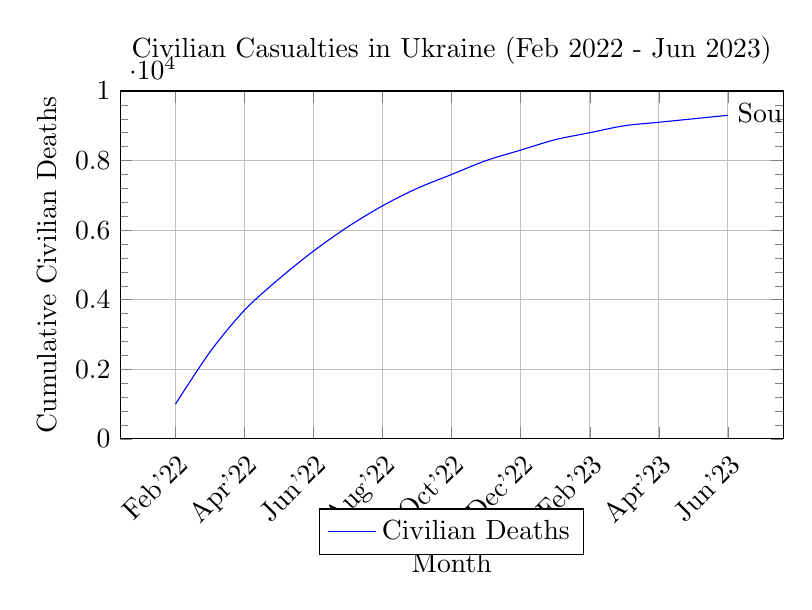
\begin{tikzpicture}
    \begin{axis}[
        title={Civilian Casualties in Ukraine (Feb 2022 - Jun 2023)},
        xlabel={Month},
        ylabel={Cumulative Civilian Deaths},
        grid=major,
        width=10cm,
        height=6cm,
        xtick={1,3,5,7,9,11,13,15,17},
        xticklabels={Feb'22,Apr'22,Jun'22,Aug'22,Oct'22,Dec'22,Feb'23,Apr'23,Jun'23},
        xticklabel style={rotate=45,anchor=north east},
        ymin=0,
        ymax=10000,
        minor y tick num=4,
        legend style={at={(0.5,-0.2)},anchor=north}
    ]
    \addplot[smooth,mark=none,blue] coordinates {
        (1, 1000) (2, 2500) (3, 3700) (4, 4600) (5, 5400) 
        (6, 6100) (7, 6700) (8, 7200) (9, 7600) (10, 8000) 
        (11, 8300) (12, 8600) (13, 8800) (14, 9000) (15, 9100) 
        (16, 9200) (17, 9300)
    };
    \legend{Civilian Deaths}
    \node at (axis cs:17,9300) [anchor=west] {Source: UN OHCHR \cite{un_2023}};
    \end{axis}
\end{tikzpicture}

\vspace{1cm}

% Grafic 2: Refugiați
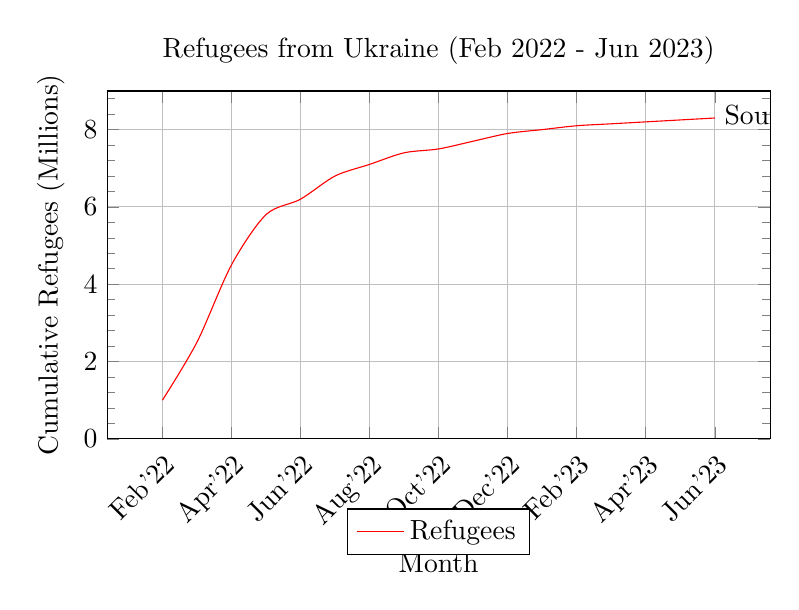
\begin{tikzpicture}
    \begin{axis}[
        title={Refugees from Ukraine (Feb 2022 - Jun 2023)},
        xlabel={Month},
        ylabel={Cumulative Refugees (Millions)},
        grid=major,
        width=10cm,
        height=6cm,
        xtick={1,3,5,7,9,11,13,15,17},
        xticklabels={Feb'22,Apr'22,Jun'22,Aug'22,Oct'22,Dec'22,Feb'23,Apr'23,Jun'23},
        xticklabel style={rotate=45,anchor=north east},
        ymin=0,
        ymax=9,
        minor y tick num=4,
        legend style={at={(0.5,-0.2)},anchor=north}
    ]
    \addplot[smooth,mark=none,red] coordinates {
        (1, 1) (2, 2.5) (3, 4.5) (4, 5.8) (5, 6.2) 
        (6, 6.8) (7, 7.1) (8, 7.4) (9, 7.5) (10, 7.7) 
        (11, 7.9) (12, 8.0) (13, 8.1) (14, 8.15) (15, 8.2) 
        (16, 8.25) (17, 8.3)
    };
    \legend{Refugees}
    \node at (axis cs:17,8.3) [anchor=west] {Source: UNHCR \cite{unhcr_2023}};
    \end{axis}
\end{tikzpicture}
 % Include grafice victime și refugiați
\end{center}

These consequences underscore the war’s far-reaching impact, not only on Ukraine but on global stability and human dignity. The failure to address these costs perpetuates a cycle of suffering and instability.

\section{Manifesto for Action}
The blood spilled in Ukraine cries out for more than reports and resolutions—it demands action, fierce and unwavering. The scale of atrocities and the erosion of global norms compel us to propose a roadmap for justice, humanity, and renewal. These are not mere suggestions; they are imperatives for a world that dares to call itself civilized \cite{icc_2023, un_inquiry_2023}.

\begin{itemize}
    \item \textbf{Establish an International Tribunal for Russian War Crimes}: A dedicated tribunal, under UN auspices or a coalition of willing states, must prosecute those responsible for war crimes, crimes against humanity, and genocide in Ukraine. The ICC’s arrest warrants for Putin and Lvova-Belova are a start, but a specialized court would accelerate justice and amplify global legitimacy \cite{icc_2023}.
    
    \textit{Why it matters}: Every unpunished massacre—from Bucha to Mariupol—emboldens tyrants. Justice is not a luxury; it is the foundation of peace.

    \item \textbf{Apply Coordinated Diplomatic Pressure}: The EU, NATO, and G7 must unite to isolate Russia politically—expelling it from international forums like the G20 and challenging its UN Security Council veto, a grotesque privilege for a state that defies the UN Charter \cite{un_charter}.
    
    \textit{Why it matters}: Diplomacy without teeth is a hollow gesture. Silence in the face of aggression is betrayal.

    \item \textbf{Increase Humanitarian and Defensive Support to Ukraine}: Ukraine needs more than weapons; it needs medicine, shelter, and hope for millions displaced. Military aid must include air defense systems and long-range capabilities, delivered swiftly and without restrictive conditions, to protect civilians and reclaim sovereignty \cite{unhcr_2023}.
    
    \textit{Why it matters}: A mother shielding her child from bombs does not care for geopolitics. Support is not escalation—it is humanity.

    \item \textbf{Launch Independent Monitoring Missions in Occupied Territories}: Deploy OSCE or neutral observers to document abuses in real-time, from torture to forced deportations, ensuring truth survives the fog of war \cite{osce_2023}.
    
    \textit{Why it matters}: Every hidden crime is a wound unhealed. Transparency is the enemy of impunity.

    \item \textbf{Invest in Sustainable Reconstruction}: Ukraine’s rebirth must be green, resilient, and just. A global fund, led by the EU and World Bank, should finance energy-independent cities, restored ecosystems, and infrastructure built for the future, not the past \cite{world_bank_2023, eco_impact_2023}.
    
    \textit{Why it matters}: To rebuild is to defy destruction. Ukraine’s recovery is a testament to human resolve.
\end{itemize}

\subsection*{Final Appeal}
This is not a crisis for diplomats alone—it is a reckoning for every soul who values life over apathy. The screams of Ukraine’s children, the grief of its families, and the defiance of its people echo in our collective conscience. Silence is not neutrality; it is complicity. To ignore this war is to forsake our shared humanity. History will remember not only those who acted, but also those who remained silent.

We call on leaders to act with courage, not caution. We call on citizens—across borders, faiths, and futures—to demand justice, to amplify truth, to stand with the violated. Raise your voice. Share this truth. Hold power accountable. The blood in Ukraine stains us all until we act.

This manifesto is a vow: we will not look away. We will not forget. We will fight for a world where no child’s life is a bargaining chip, no nation’s sovereignty a footnote. Join us. The time for action is now.

\section{Dedication}
This report is dedicated to the victims of Russia’s war on Ukraine—those who have lost their lives, their homes, and their futures. Their resilience inspires us, and their suffering demands our action. We also extend gratitude to the global community—activists, volunteers, and ordinary citizens—who have stood in solidarity with Ukraine, proving that humanity can triumph over indifference. May this work honor their courage and contribute to a just future.

\printbibliography

\end{document}
